\section{Durchführung}
\subsection{Gedämpfte Schwingung}
In dem Stromkreis \ref{fig:d1} wird ein einzelner Strompuls in Form
von Rechteckwechselspannung simuliert, sodass die
abnehmenden Amplituden der Spannungskurve nach der Zeit von dem Osziloskop abgelesen werden können.
\label{sec:Durchführung}
\begin{figure}[H]
  \centering
  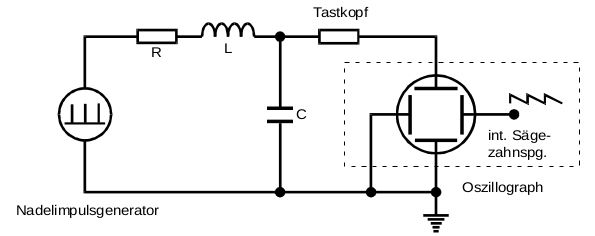
\includegraphics{content/images/d1.png}
  \caption{Schaltkreis gedämpfte Schwingung experimentell.}
  \label{fig:d1}
\end{figure}

\subsection{aperiodischer Grenzfall}
Bei erneutem einspeisen einer Rechteckwechselspannung in \ref{fig:d2} wird der verstellbare
Widerstand so eingestellt, dass gerade kein Überschwingen mehr
vom Osziloskop abzulesen ist.
\begin{figure}[H]
  \centering
  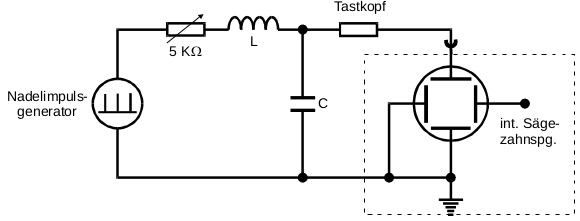
\includegraphics{content/images/d2.png}
  \caption{Schaltkreis Bestimmung des aperiodischen Grenzfalls experimentell.}
  \label{fig:d2}
\end{figure}

\subsection{Frequenzabhängige Kondensatorspannung}
\label{sec:d3}
Die Kondensatorspannung in \ref{fig:d3} wird für verschiedene Frequenzen abgelesen bis sich ein
Maximum an der Eigenfrequenz des Schwingkreises gebildet hat.
\begin{figure}[H]
  \centering
  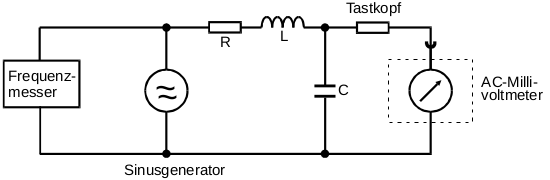
\includegraphics{content/images/d3.png}
  \caption{Schaltkreis Kondensatorspannung zu Frequenz experimentell.}
  \label{fig:d3}
\end{figure}

\subsection{Frequenzabhängige Phase}
Erreger- und Kondensatorspannung in \ref{fig:d4} werden auf dem Oszilloskop übereinander gelegt
und die Phasendifferenz wird auf dem selben Intervall wie in \ref{sec:d3} notiert.
\begin{figure}[H]
  \centering
  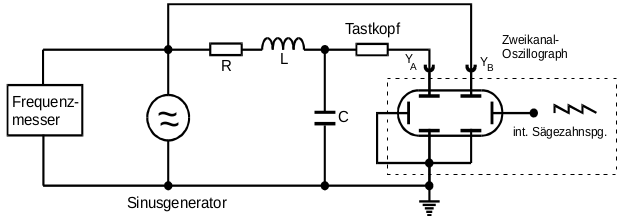
\includegraphics{content/images/d4.png}
  \caption{Schaltkreis Phase zwischen Erreger- und Kondensatorspannung zu Frequenz experimentell.}
  \label{fig:d4}
\end{figure}
